\documentclass[tikz,border=2pt]{standalone}
\usepackage{amsmath,amssymb}
\usepackage{tikz}

\begin{document}
% An open cover of the segment E = [0,1]: overlapping open intervals (patches) whose union
% contains E. Here five patches suffice (a finite subcover).
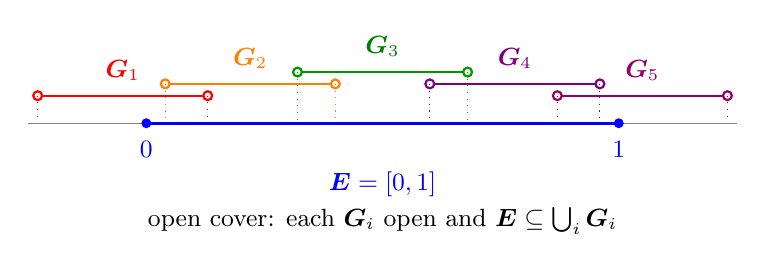
\begin{tikzpicture}[x=6cm, every node/.style={font=\small}]
	\draw[gray] (-0.25,0) -- (1.25,0);
	\draw[very thick, blue] (0,0) -- (1,0);
	\fill[blue] (0,0) circle (1.8pt) node[below=3pt] {$0$};
	\fill[blue] (1,0) circle (1.8pt) node[below=3pt] {$1$};
	\node[blue, below=14pt] at (0.5,0) {$\boldsymbol{E}=[0,1]$};
	\foreach \c/\h/\col in {-0.05/0.35/red, 0.22/0.5/orange, 0.5/0.65/green!60!black, 0.78/0.5/violet, 1.05/0.35/red!60!blue} {
		\draw[\col, thick] ({\c-0.18},\h) -- ({\c+0.18},\h);
		\draw[\col, thick, fill=white] ({\c-0.18},\h) circle (1.6pt);
		\draw[\col, thick, fill=white] ({\c+0.18},\h) circle (1.6pt);
		\draw[\col, dotted] ({\c-0.18},\h) -- ({\c-0.18},0.02);
		\draw[\col, dotted] ({\c+0.18},\h) -- ({\c+0.18},0.02);
	}
	\node[red, above=2pt] at (-0.05,0.35) {$\boldsymbol{G}_1$};
	\node[orange, above=2pt] at (0.22,0.5) {$\boldsymbol{G}_2$};
	\node[green!50!black, above=2pt] at (0.5,0.65) {$\boldsymbol{G}_3$};
	\node[violet, above=2pt] at (0.78,0.5) {$\boldsymbol{G}_4$};
	\node[red!60!blue, above=2pt] at (1.05,0.35) {$\boldsymbol{G}_5$};
	\node[anchor=north] at (0.5,-0.95) {open cover: each $\boldsymbol{G}_i$ open and $\boldsymbol{E}\subseteq\bigcup_i\boldsymbol{G}_i$};
\end{tikzpicture}
\end{document}
